% Options for packages loaded elsewhere
\PassOptionsToPackage{unicode}{hyperref}
\PassOptionsToPackage{hyphens}{url}
\PassOptionsToPackage{dvipsnames,svgnames,x11names}{xcolor}
%
\documentclass[
  authoryear]{elsarticle}

\usepackage{amsmath,amssymb}
\usepackage{iftex}
\ifPDFTeX
  \usepackage[T1]{fontenc}
  \usepackage[utf8]{inputenc}
  \usepackage{textcomp} % provide euro and other symbols
\else % if luatex or xetex
  \usepackage{unicode-math}
  \defaultfontfeatures{Scale=MatchLowercase}
  \defaultfontfeatures[\rmfamily]{Ligatures=TeX,Scale=1}
\fi
\usepackage{lmodern}
\ifPDFTeX\else  
    % xetex/luatex font selection
\fi
% Use upquote if available, for straight quotes in verbatim environments
\IfFileExists{upquote.sty}{\usepackage{upquote}}{}
\IfFileExists{microtype.sty}{% use microtype if available
  \usepackage[]{microtype}
  \UseMicrotypeSet[protrusion]{basicmath} % disable protrusion for tt fonts
}{}
\makeatletter
\@ifundefined{KOMAClassName}{% if non-KOMA class
  \IfFileExists{parskip.sty}{%
    \usepackage{parskip}
  }{% else
    \setlength{\parindent}{0pt}
    \setlength{\parskip}{6pt plus 2pt minus 1pt}}
}{% if KOMA class
  \KOMAoptions{parskip=half}}
\makeatother
\usepackage{xcolor}
\setlength{\emergencystretch}{3em} % prevent overfull lines
\setcounter{secnumdepth}{5}
% Make \paragraph and \subparagraph free-standing
\ifx\paragraph\undefined\else
  \let\oldparagraph\paragraph
  \renewcommand{\paragraph}[1]{\oldparagraph{#1}\mbox{}}
\fi
\ifx\subparagraph\undefined\else
  \let\oldsubparagraph\subparagraph
  \renewcommand{\subparagraph}[1]{\oldsubparagraph{#1}\mbox{}}
\fi


\providecommand{\tightlist}{%
  \setlength{\itemsep}{0pt}\setlength{\parskip}{0pt}}\usepackage{longtable,booktabs,array}
\usepackage{calc} % for calculating minipage widths
% Correct order of tables after \paragraph or \subparagraph
\usepackage{etoolbox}
\makeatletter
\patchcmd\longtable{\par}{\if@noskipsec\mbox{}\fi\par}{}{}
\makeatother
% Allow footnotes in longtable head/foot
\IfFileExists{footnotehyper.sty}{\usepackage{footnotehyper}}{\usepackage{footnote}}
\makesavenoteenv{longtable}
\usepackage{graphicx}
\makeatletter
\def\maxwidth{\ifdim\Gin@nat@width>\linewidth\linewidth\else\Gin@nat@width\fi}
\def\maxheight{\ifdim\Gin@nat@height>\textheight\textheight\else\Gin@nat@height\fi}
\makeatother
% Scale images if necessary, so that they will not overflow the page
% margins by default, and it is still possible to overwrite the defaults
% using explicit options in \includegraphics[width, height, ...]{}
\setkeys{Gin}{width=\maxwidth,height=\maxheight,keepaspectratio}
% Set default figure placement to htbp
\makeatletter
\def\fps@figure{htbp}
\makeatother

\makeatletter
\@ifpackageloaded{caption}{}{\usepackage{caption}}
\AtBeginDocument{%
\ifdefined\contentsname
  \renewcommand*\contentsname{Table of contents}
\else
  \newcommand\contentsname{Table of contents}
\fi
\ifdefined\listfigurename
  \renewcommand*\listfigurename{List of Figures}
\else
  \newcommand\listfigurename{List of Figures}
\fi
\ifdefined\listtablename
  \renewcommand*\listtablename{List of Tables}
\else
  \newcommand\listtablename{List of Tables}
\fi
\ifdefined\figurename
  \renewcommand*\figurename{Figure}
\else
  \newcommand\figurename{Figure}
\fi
\ifdefined\tablename
  \renewcommand*\tablename{Table}
\else
  \newcommand\tablename{Table}
\fi
}
\@ifpackageloaded{float}{}{\usepackage{float}}
\floatstyle{ruled}
\@ifundefined{c@chapter}{\newfloat{codelisting}{h}{lop}}{\newfloat{codelisting}{h}{lop}[chapter]}
\floatname{codelisting}{Listing}
\newcommand*\listoflistings{\listof{codelisting}{List of Listings}}
\makeatother
\makeatletter
\makeatother
\makeatletter
\@ifpackageloaded{caption}{}{\usepackage{caption}}
\@ifpackageloaded{subcaption}{}{\usepackage{subcaption}}
\makeatother
\journal{JIMR}
\ifLuaTeX
  \usepackage{selnolig}  % disable illegal ligatures
\fi
\usepackage[]{natbib}
\bibliographystyle{elsarticle-harv}
\usepackage{bookmark}

\IfFileExists{xurl.sty}{\usepackage{xurl}}{} % add URL line breaks if available
\urlstyle{same} % disable monospaced font for URLs
\hypersetup{
  pdftitle={Beyond the paradox of interoperability in open health data standards},
  pdfauthor={Daniel Kapitan; Melle Sieswerda; Bart-Jan Verhoeff; XXX; Andre Dekker},
  pdfkeywords={OMOP, OpenEHR, FHIR, secondary use, data
platform, digital platform},
  colorlinks=true,
  linkcolor={blue},
  filecolor={Maroon},
  citecolor={Blue},
  urlcolor={Blue},
  pdfcreator={LaTeX via pandoc}}

\setlength{\parindent}{6pt}
\begin{document}

\begin{frontmatter}
\title{Beyond the paradox of interoperability in open health data
standards}
\author[1,2,3]{Daniel Kapitan%
%
}
 \ead{daniel@kapitan.net} 
\author[4,5]{Melle Sieswerda%
%
}

\author[6]{Bart-Jan Verhoeff%
%
}

\author[2]{XXX%
%
}

\author[5]{Andre Dekker%
%
}


\affiliation[1]{organization={Dutch Hospital
Data},city={Utrecht},country={the
Netherlands},countrysep={,},postcodesep={}}
\affiliation[2]{organization={PharmAccess
Foundation},city={Amsterdam},country={the
Netherlands},countrysep={,},postcodesep={}}
\affiliation[3]{organization={Eindhoven University of
Technology},city={Eindhoven},country={the
Netherlands},countrysep={,},postcodesep={}}
\affiliation[4]{organization={Integral Cancer Registry
Netherlands},city={Eindhoven},country={the
Netherlands},countrysep={,},postcodesep={}}
\affiliation[5]{organization={Maastricht
University},city={Maastricht},country={the
Netherlands},countrysep={,},postcodesep={}}
\affiliation[6]{organization={Expertisecentrum
Zorgalgoritmen},city={Utrecht},country={the
Netherlands},countrysep={,},postcodesep={}}

\cortext[cor1]{Corresponding author}





        
\begin{abstract}
In response to the proposal of Tsafnat et al.~to converge towards three
open health data standards, this viewpoint provides a critical
reflection on the proposed alignment of using OpenEHR, FHIR and OMOP as
the default standards for clinical care and administration, data
exchange and longitudinal analysis, respectively. We argue that besides
the focus on open standards, we need to consider the ecosystem of open
source implementations in choosing an appropriate standard for a given
context. We discuss two specific contexts, namely standardization of i)
health data for federated learning, and ii) health data sharing in low-
and middle income countries (LMICs). Specific design principles,
practical considerations and implementation choices for these two
context are described, based on ongoing work in both areas. In both
cases, we observe a strong convergence towards FHIR as the primary
standard, while OMOP and OpenEHR are currently {[}\ldots some word
\ldots{]}. We propose a number of additional points to guide
developments in this area.
\end{abstract}





\begin{keyword}
    OMOP \sep OpenEHR \sep FHIR \sep secondary use \sep data
platform \sep 
    digital platform
\end{keyword}
\end{frontmatter}
    
\section{Looking beyond the paradox of
interoperability}\label{looking-beyond-the-paradox-of-interoperability}

``A paradox of health care interoperability is the existence of a large
number of standards exists with significant overlap among them,'' say
Tsafnat et al., followed by a call to actions towards the health
informatics community to put effort into establishing convergence and
preventing collision \citep{tsafnat2024converge}. To do so, they propose
to converge on three open standards, namely i) OpenEHR for clinical care
and administration; ii) Fast Health Interoperability Resources (FHIR)
for data exhange and iii) Observational Medical Outcomes Partnership
Common Data Model (OMOP) for longitudinal analysis. They argue that open
data standards, backed by engaged communities, hold an advantage over
proprietary ones and therefore should be chosen as the steppingstones
towards achieving true interoperability.

While we support their high-level rationale and intention, we feel their
proposed trichotomy does not do justice to details that are crucial in
real-world implementations. This viewpoint provides a critical
reflection on the their proposed framework in three parts. First, we
reflect on salient differences between the three open standards from the
perspective of the notion of openness of digital platforms
\citep{dereuver2018digital} and the paradox of open
\citep{keller2021paradox}. Subsequently, we present our findings in
designing and implementing health data platforms in two specific
contexts, namely i) platforms for federated learning on shared health
data; and ii) health data platforms for low and middle income countries
(LMICs). We conclude with \ldots{}

\section{The paradox of open for health data
standards}\label{the-paradox-of-open-for-health-data-standards}

Besides the paradox of interoperability put forward by Tsafnat et al.,
we argue that open standards are a necessary, but not sufficient
condition for convergence of health data standarization. We posit that
open source implementations of components, libraries etc. constitute
another necessary condition for establishing a flourishing health data
sharing platform and associated ecosystem for any given context, be it
regional, international or within a specific sub-domain like pandemic
preparedness. Research on digital platforms underline the importance of
the platform openness, not only in term of open standards, but also in
term of extensibility of the code base, availibility of complements to
the core technical platform (in our case the data standard itself) and
availibility of executable pieces of software
\citep{dereuver2018digital}. Only when the majority of these aspects of
digital platforms are fullfilled can we resonably expect that the
platform will indeed be longlived.

In what they call the paradox of open, Keller and Tarkowsi argue that
this conventional approach of open standards and open source flourish
under two types of conditions \citep{keller2021paradox}. First, projects
where many people contribute to the creation of a common resource have
proven succesful. This is the story of Wikipedia, OpenStreetMap,
Blender.org, and the countless free software projects that provide much
of the internet's infrastructure. Indeed, Tsafnat et al.~have explicitly
taken into account that ``an engaged and vibrant community is a major
advantage for the longevity of the data standards it uses,'' which has
informed their proposal to converge towards OMOP, FHIR en OpenEHR.
However, the emphasis on open source implementations is somewhat
overlooked. This point is only mentioned in passing and indirectly, when
Tsafnat et al.~reference work done by Reynolds and Wyatt who already
argued in 2011 ``\ldots{} for the superiority of open source licensing
to promote safer, more effective health care information systems. We
claim that open source licensing in health care information systems is
essential to rational procurement strategy'' \citep{reynolds2011open}.
We believe that a realistic assessment of the current position of an
open standard within the wider context of availability of complementary
components and open source implementations is equally important when
choosing which standard to adopt.

This point is related to the second condition put forward by Keller and
Tarkoswki, namely that the conventional open approach has proven
fruitful when ``opening up'' is the result of external incentives or
requirements, rather than voluntary actions. This is the story of
publicly-funded knowledge production like Open Access academic
publications, cultural heritage collections in the Public Domain, Open
Educational Resources (OER), and Open Government data. A canonical
example in the birth of the GSM standard, which was mandated by European
legislation.\footnote{See
  \url{https://en.wikipedia.org/wiki/GSM\#Initial_European_development}
  for details.} Reflecting on this perspective on openness, we observe a
salient difference between FHIR vis-a-vis OpenEHR and OMOP, namely that
the former is the only one that has been mandated (or at least strongly
recommended) in some jurisdictions. In the US, the Office of the
National Coordinator for Health Information Technology (ONC) and the
Centers for Medicare and Medicaid Services (CMS) has introduced a steady
stream of new regulations, criteria, and deadlines in Health IT that has
resulted in significant adoption of FHIR \citep{firely2023fhir}. In
India, the open Health Claims Exchange protocol specification - which is
based on FHIR - has been mandated by the Indian government as the
standard for e-claims handling \citep{india2020national, hcx}. The
African Union recommends all new implementations and digital health
system improvements use FHIR as the primary mechanism for data exchange
\citep{tilahun2023african}, but doesn't say anything about the use of,
for example, OpenEHR for administrative point-of-service systems.

These external incentives have resulted in a large boost in both
commercial and open source development activities in the FHIR ecosystem.
One such example is the speed with which the Bulk FHIR API has been
defined and implemented in almost all major implementations
\citep{mandl2020push, jones2021landscape}. It has also led to more
people voluntarily contributing to FHIR-related open source projects,
which has resulted in a wide offering of FHIR components across major
technology stacks (Java, Python, .NET), thereby strengthening the first
condition. By comparison, OMOP and OpenEHR have not yet profited from
external incentives to spur the adoption and thereby growing the
ecosystem beyond a certain critical mass. To illustrate this, a search
on GitHub on ``FHIR'' yields 8.2 thousand results, ``OMOP or OHDSI'' one
thousand results, and ``OpenEHR'' yiels 400 results.

\begin{itemize}
\tightlist
\item
  The majority of OMOP components are run by Observational Health Data
  Science and Informatics (OHDSI) \ldots Say something that OMOP still
  has a relatively large ecosystem, with R libraries, pyOMOP etc.
\item
  The OpenEHR, however, seems subscritical. We are not judging the
  content and approach of OpenEHR, but there are just so few
  implementations.
\end{itemize}

Hence, we stress that beyond the evaluating the instrinic structure of
an open standard and the community that supports the standard, we need
to take into account the wider ecosystem of open source implementations,
complementary components etc. From this wider perspective on the whole
ecosystem around a standard, FHIR stands out as having the diverse and
rich ecosystem because it has been mandated in certain jurisdictions.
This is relevant when comparing these standards in real-world
implementations. We now turn to two specific use cases c.q. contexts
where these considerations are at play.

\section{Standarization of health data for federated
learning}\label{standarization-of-health-data-for-federated-learning}

The current fragmentation in health data is one of the major barriers
towards leveraging the potential medical data for machine learning (ML).
Without access to sufficient data, ML will be prevented from reaching
its full potential and, ultimately, from making the transition from
research to clinical practice. Data like this is hard to obtain, because
health data is highly sensitive and its usage is tightly regulated.

Federated learning (FL) is a learning paradigm that aims to address
these issues of data governance and privacy by training algorithms
collaboratively without exchanging the data itself
\citep{rieke2020future, teo2024federated}. Based on ongoing work with
the PLUGIN healthcare consortium (\url{https://plugin.healthcare}, in
Dutch) we have detailed an architecture for FL for secondary use of
health data in the Netherlands. Starting point for this implementation
are the National Health Data Infrastructure agreements for research,
policy and innovation for the Dutch healthcare sector, which have been
adopted at the beginning of 2024 \citep{healthri2024agreements}.
Figure~\ref{fig-healthri-architecture} shows a high level overview of
the platform, which comprises three areas (multiple use, applications
and generic features) and a total of 26 functional components (for
details please refer to \citep{healthri2024agreements}).

\begin{figure}

\centering{

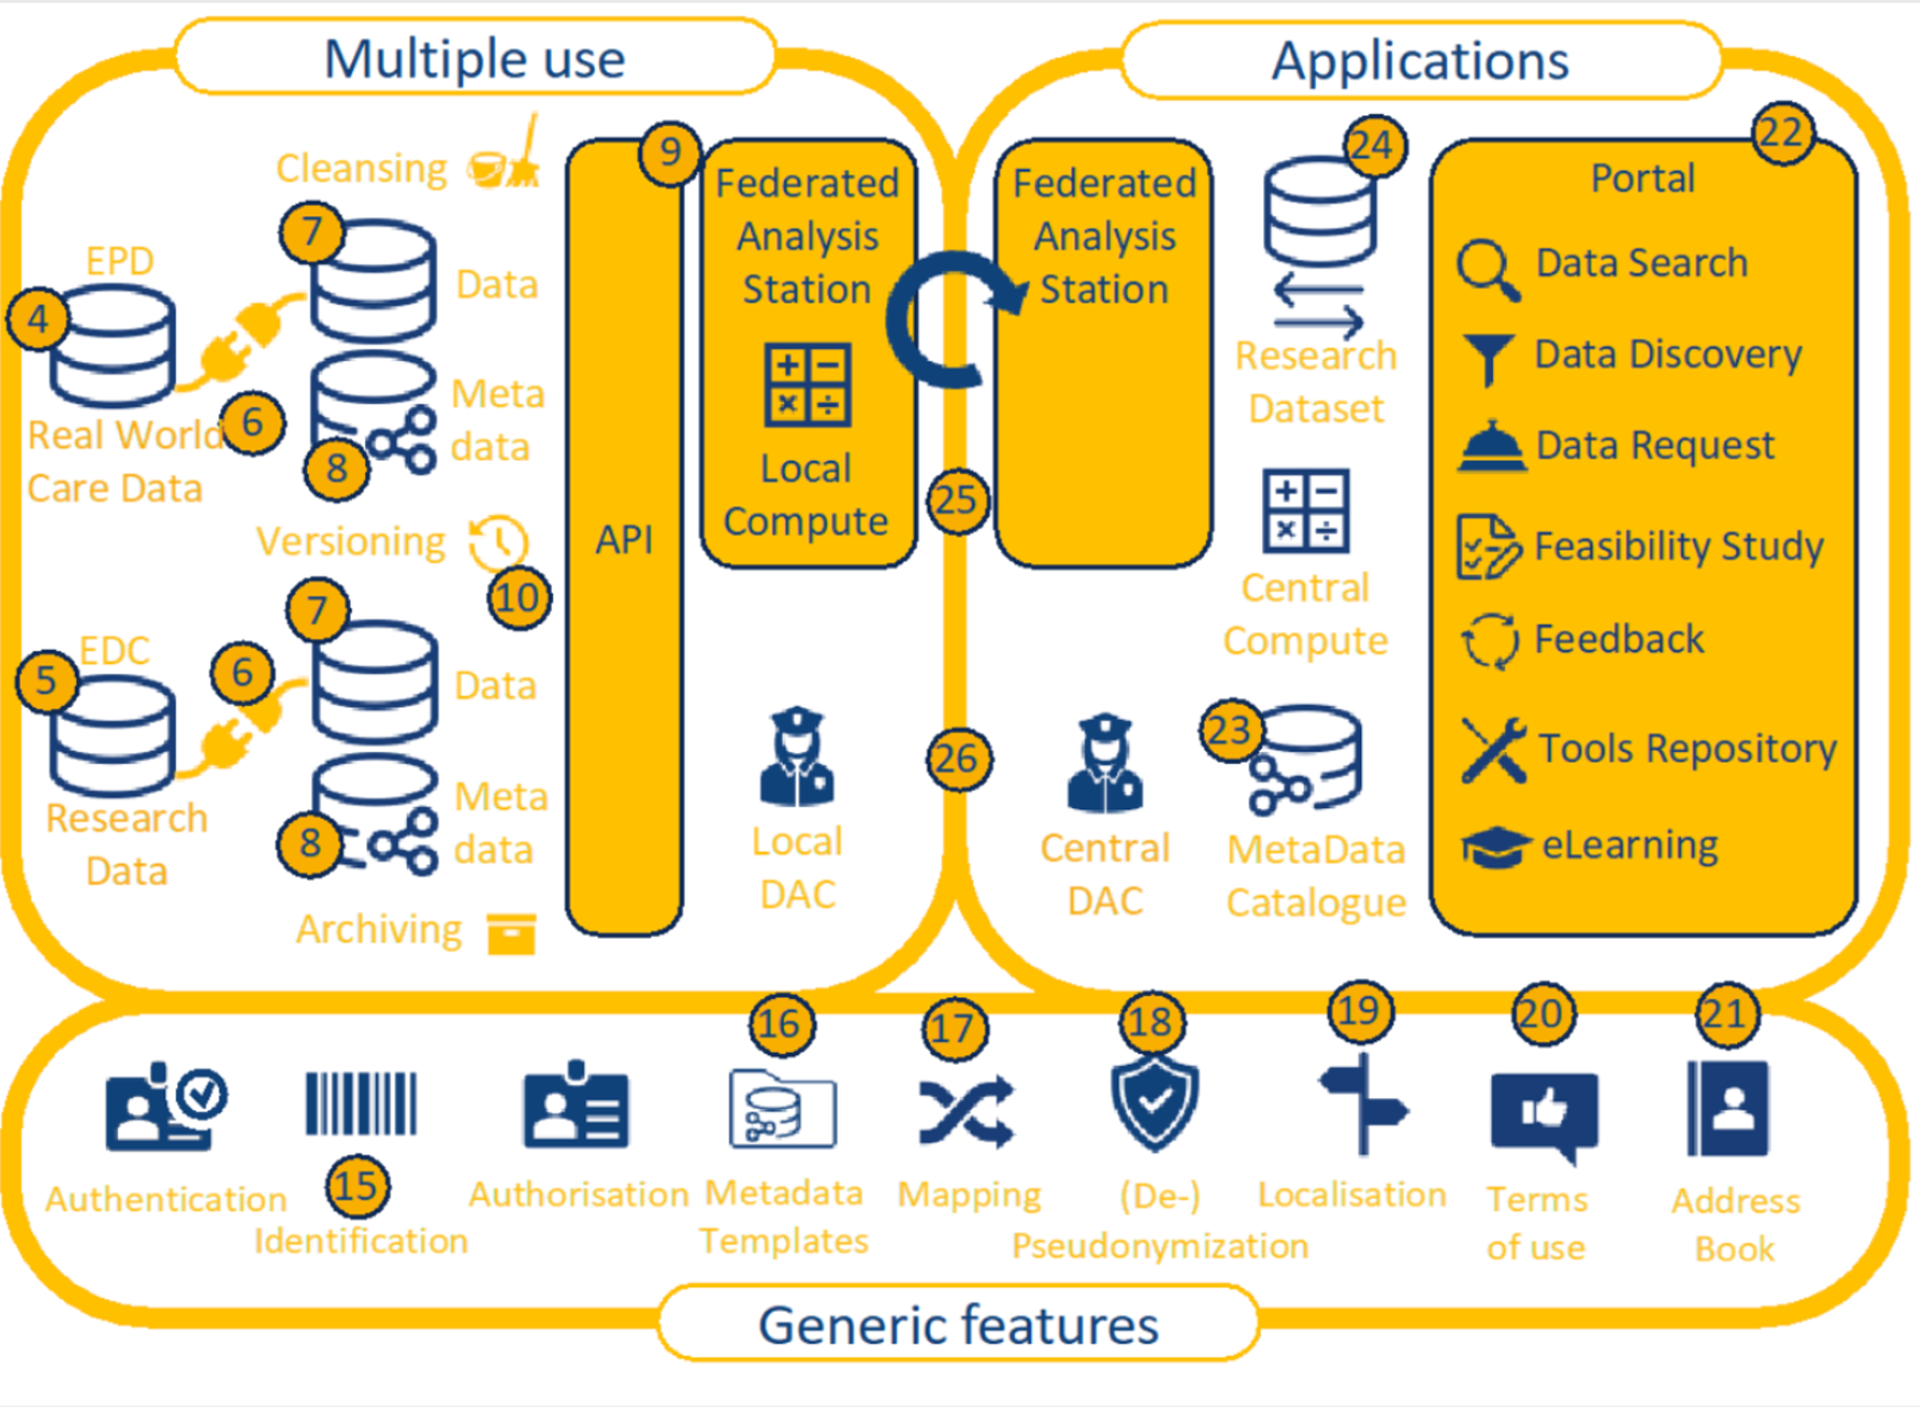
\includegraphics{health-ri-architecture.png}

}

\caption{\label{fig-healthri-architecture}Reference architecture for the
Dutch health data infrastructure for research and innovation
\citep{healthri2024agreements}}

\end{figure}%

The principle of FL has been actively researched and developed within
the Dutch healthcare community. The first proof-of-concept of the
so-called Personal Health Train \citep{vansoest2018using} ultimately led
to the open source vantage6 platform \citep{smits2022improved}. One of
the prerequisites of this architecture is that organizations that
participate in a federation of `data stations' use the same common data
model to make the data Findable, Accessible, Interoperable and Resusable
(FAIR). These FAIR data stations comprise components 7, 8 and 9 in
Figure~\ref{fig-healthri-architecture}, i.e.~the data, metadata and
APIs, respectively, through which this the data station can be accessed
and used. FHIR has been chosen as the common data model quite early in
the development because of its practicality, provenance of RESTful APIs
out of the box, support of many healthcare terminologies and flexibility
through the profiling mechanims \citep{choudhury2020personal}. This
solution design has gained traction since then. The CODA platform, which
aims to implement a similar FL infrastructure in Canada, compared OMOP
and FHIR and chose the latter as it has been found to support more
granular mappings required for analytics \citep{mullie2023coda}. The
fair4health project has implemented also based on FHIR, but using a
different open source framework for federated learning
\citep{sinaci2024privacypreserving}.

Using the FHIR standard for persistent storage for longitudinal data in
such FL architectures may strike many as counterintuitive. Another
common approache takes OMOP as the the common data model more in line
with the proposal of Tsafnat et al.~Reports of real-world
implementations based on the OHDSI-OMOP stack include a global
infrastructure with 22 centres for COVID19 prediction
models\citep{khalid2021standardized}, FeederNet in South Korea with 57
participating hospitals \citep{lee2022feedernet}, Dutch multi-cohor
dementia research with 9 centres \citep{mateus2024data}, the European
severe heterogeneous asthma research collaboration
\citep{kroes2022blueprint}.

Given that conceptually OMOP can be viewed as a strict subset of FHIR,
hybrid solutions using OMOP and FHIR combined have also been reported,
such as the German KETOS platform \citep{gruendner2019ketos}, and the
preliminary findings from the European GenoMed4All project which aims to
connect clinical and -omics data \citep{cremonesi2023need}. A
collaboration of 10 university hospitals in Germany have shown that
standardized ETL-processing from FHIR into OMOP can achieve 99\%
conformance \citep{peng2023etlprocess}, which confirms the feasiblity of
the solution pattern where FHIR acts as an intermediate sharing standard
through which data from (legacy) systems are extracted and made
available for reuse in a common data model.

One could argue that the distiction between FHIR amd OMOP becomes less
relevant if data can be effectively stored in either standard. We are
hopeful that initiatives like https://omoponfhir.org indeed will foster
convergence rather than collision between these two standards. In the
case of PLUGIN, however, we had other considerations to opt for FHIR.

First, we find that the mechanism of FHIR Profiles can be tied to
concept of late binding commonly applied in data lake/warehouse
architectures: allow ingest of widely different sources, and gradually
but more constraints and validations as you move closer to a specific
use case. If machine learning is the primary objective for secondary
use, we want to be able to cast a wider net of relevant data, rather
than having very detailed data. Late binding in data warehousing is a
design philosophy where data transformation and schema enforcement are
deferred until as late as possible in the data processing pipeline,
sometime even until query time. This approach contrasts with early
binding, where data is transformed and structured as it is ingested into
the data warehouse. Put differently, we defer from transforming data at
the point of ingestion (ETL - Extract, Transform, Load), but rather
apply transformations when the data is accessed for analysis (ELT -
Extract, Load, Transform).

FHIR Profiles are a key mechanism for defining, constraining, and
extending FHIR resources to meet specific use cases and requirements in
healthcare data exchange. We FHIR Profiles to create increasingly more
strict standardized data models to ensure consistent and accurate data
representation across the various use-cases. Combining this mechanism
with late binding, we use a solution pattern whereby the zones of the
lakehouse (more on that later) correspond to FHIR profiles with
increasingly more specific constraints. This principle is visualized as
concentric circles (see below).

\begin{figure}[H]

{\centering 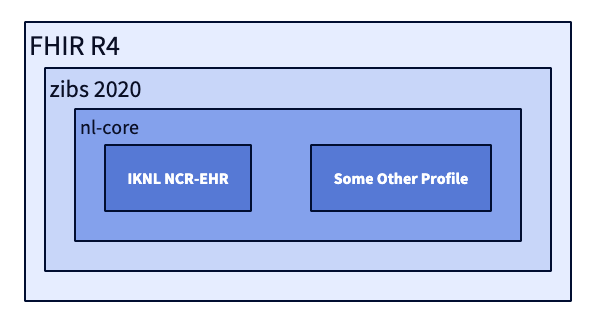
\includegraphics{late-binding.png}

}

\caption{Principle of late binding with FHIR profiling mechanism}

\end{figure}%

The advantages of this design is that it allows for greater flexibility.
During the initial ingest of the data, we only require the data to
conform to the minimal syntactic standard defined by the base FHIR
version (R4 in the diagram). As the data is processed, more strict
checks and constrains are applied, whereby ultimately different profiles
can co-exists next to one another (the two most inner circles), within a
larger circle with fewer strictions. This approach does not support the
extension mechanism of FHIR, so we need to be cautious if we decide to
use that.

The main disadvantage in using FHIR in this way pertains to the need for
upgrading the whole ELT pipeline when upgrading to a new primary FHIR
version, for example R5. However, we expect that the development time
required to upgrade FHIR versions is significantly less than the initial
migration to FHIR.

\begin{itemize}
\tightlist
\item
  Add more arguments here \ldots{[}Melle{]}
\end{itemize}

\section{Health data standards in low- and middle income
countries}\label{health-data-standards-in-low--and-middle-income-countries}

It is a widely held belief that digital technologies have an important
role to play in strengthening health systems in LMICs. Yet, also here
the current fragmentation of health data stands in the way of scaling up
digital health programme beyond project-centric, vertical solutions into
sustainable health information exchanges. And also here, many have
called to converge towards open standards \citep{mehl2023fullstac}.
Based on our direct involvement in implementing and designing health
data platforms in sub-Saharan African countries, and in line with the
approach put forward by Mehl et al., we emphasis the need for
convergence not only on i) open standards, but also on ii) open
technologies (similar to our arguments discussed in the above), iii)
open architectures (doucmentation, using open standards, of reusable
enterprise architecture patterns for health systems) and iv) open
content (representations of public health, health system or clinical
knowledge to guide implementations).

Many sub-Saharan African countries have adopted the OpenHIE framework
\citep{openhie} as the architectural blueprint for implementing
nation-wide health information exchanges (HIE) \citep{mamuye2022health},
including Nigeria \citep{dalhatu2023paper}, Kenya
\citep{thaiya2021adoption} and Tanzania \citep{nsaghurwe2021one}. While
the OpenHIE specification is agnostic to which data standard should be
used, in practice the digital health community in the global South have
\emph{de facto} converged towards FHIR as the common data model, not
only for data exchange, but also for point-of-service systems to support
clinical care and administration, and persistent, longitudinal storage
of data in the so-called Shared Health Record
\citep{ohie2023unconference}. The adoption of FHIR as the default
standard for all three domains is fueled by the widespread availibility
of open-access software infrastructure which enables and end-to-end
integration. To illustrate this, consider For example, the Open Health
Stack (OHS) consists of a new suite of digital public goods, including a
software development kit for building FHIR-native apps on Android, and
analytics tooling to generate insights from FHIR data. This solution
design blurs the distinction between the three original domains for
health data standardization.

Arguments to add:

\begin{itemize}
\tightlist
\item
  explain that we don't see OpenEHR playing any role of significance.
  Largest open source EHR implementations working with own data models.
  Unlikely this will change any time soon
  \citep{syzdykova2017opensource}
\item
  instead, we see that FHIR is in fact being adopted as a
  point-of-service system. this is possible because data is of lower
  complexity and the majority of smaller health facilities are resource
  constrained anyway --\textgreater{} moving towards a scenario where an
  app used by the health care worker is the system of record. Here we
  see a convergence of the three domains put forward by Tsafnat: the
  Shared Health Record serves as the back-end of the system-of-record,
  it provides a transactional, persistent storage engine for enabling
  information exchange and it is the longitudinal data that is used
  downstream for analytics, monitoring etc.
\item
  explain example OHS/OpenSRP: maternal care
\item
  \begin{itemize}
  \tightlist
  \item
    explain there is lot of complementatry open technologies and open
    content, to get going
  \item
    and SDK to build apps
  \item
    Clinical workflows which can be configured in a FHIR-native front-
    and backend
  \item
    InstantHIE to deploy a swarm of containers to provision all relevant
    components
  \item
    leverage open source data \& analytics components to build data
    stations/data warehouses at any scle
  \end{itemize}
\item
  also technical advantages of FHIR

  \begin{itemize}
  \tightlist
  \item
    explain that because FHIR is based on web technologies, it lends it
    self serverless implementations, separation of storage and
    compute(ref composable data stack); and downward scaleability
    (running in the browser)
  \item
    how does this relate to ontologies/graph-based? FHIR can be
    expressed in graphs \citep{gebreslassie2023fhir4fair}{]}
  \end{itemize}
\end{itemize}

\begin{figure}

\begin{minipage}{\linewidth}

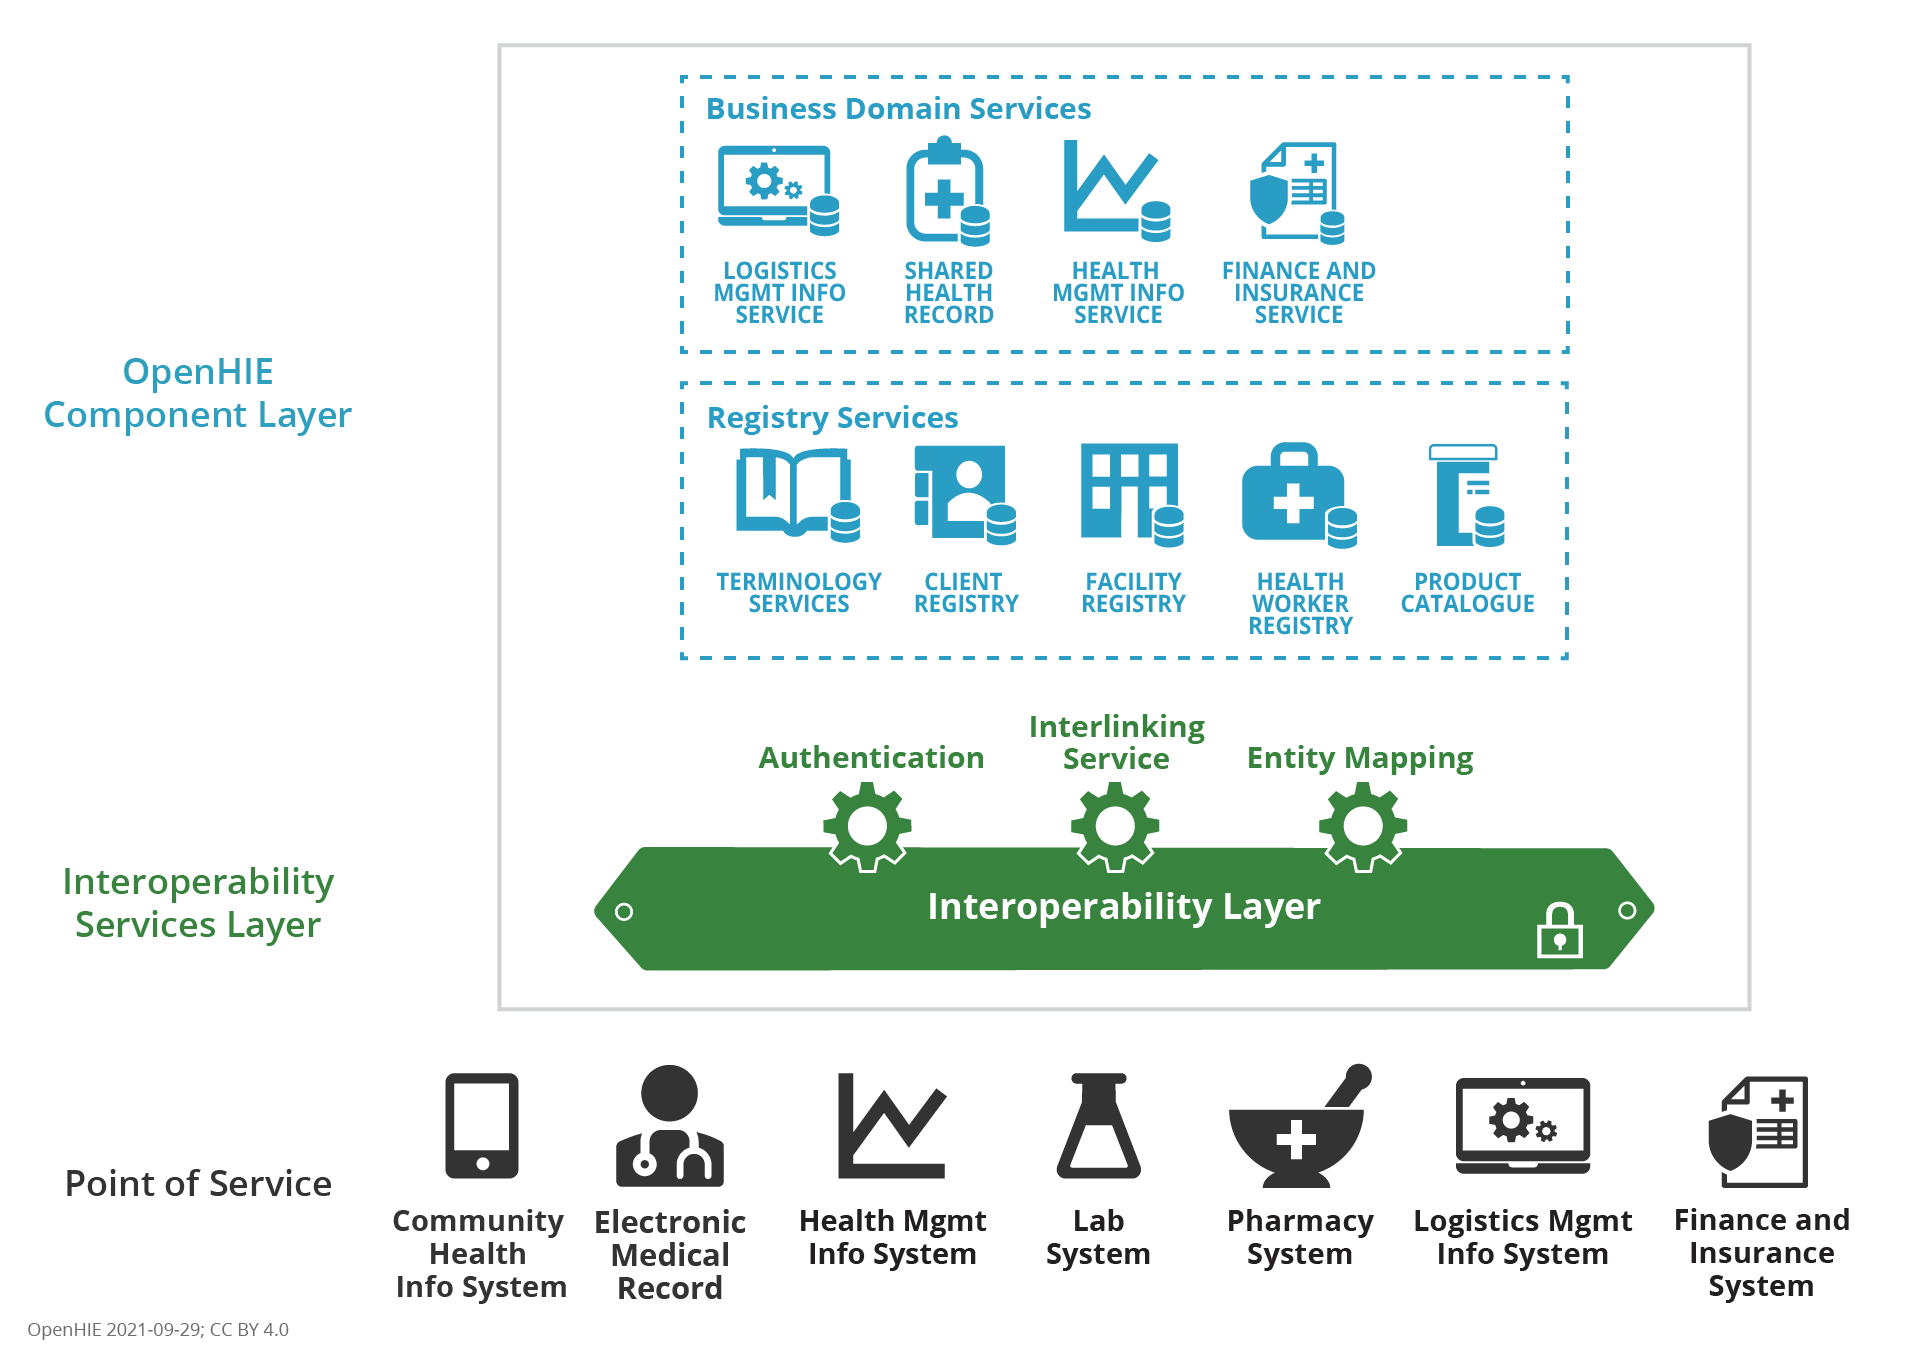
\includegraphics{openhie.png}

\subcaption{\label{}a)}
\end{minipage}%
\newline
\begin{minipage}{\linewidth}

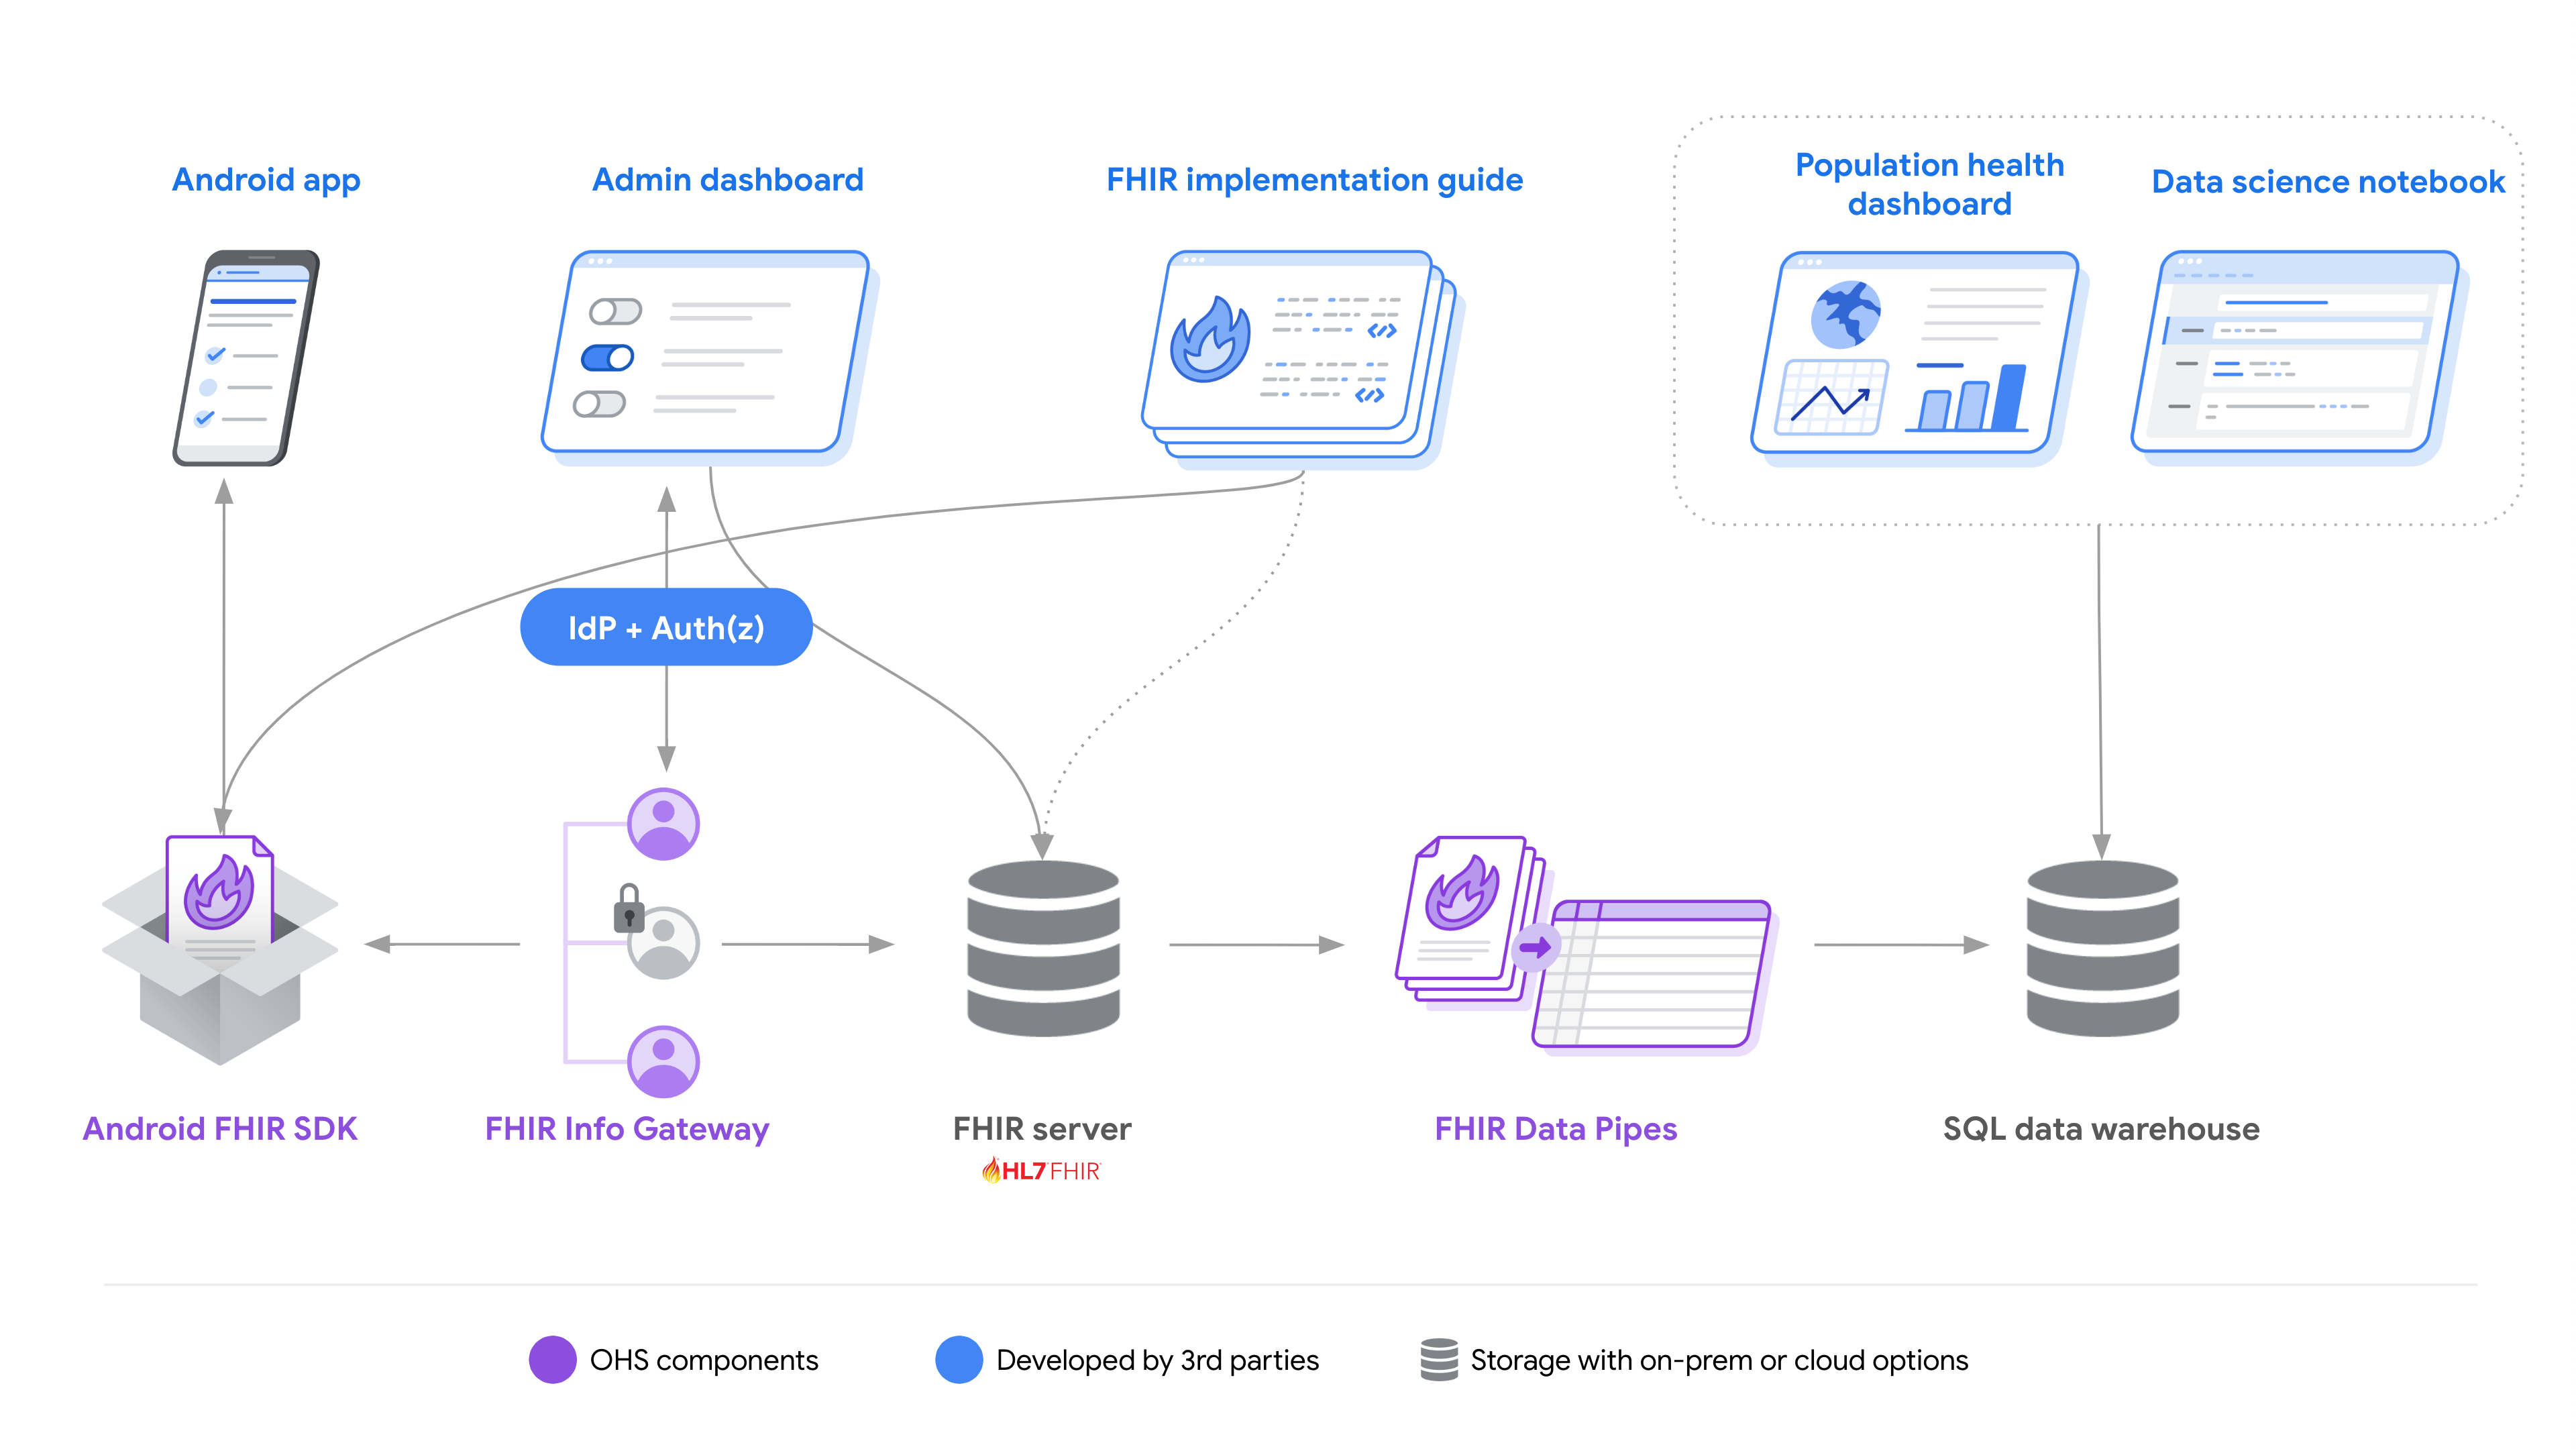
\includegraphics{ohs-endtoend.png}

\subcaption{\label{}b)}
\end{minipage}%

\caption{\label{fig-openhie}The OpenHIE reference architecture (a) and
themain components in the Open Health Stack (b).}

\end{figure}%

\section{Conclusion and outlook}\label{conclusion-and-outlook}

\begin{itemize}
\tightlist
\item
  We underline the need for open data standards as a necessary condition
  to achieve interoperability
\item
  It is not a sufficient condition
\item
  Suggestion: can we maken OMOP and OpenEHR benefit from the open
  technologies on FHIR? We think that through making open source
  reference implementations, such as OMOP-on-FHIR (what's EHR equivalent
  of that?) we can
\item
  MPC as next step up from FL
\item
  More than a decade later, we observe that only a very small fraction
  of health IT systems are based on open source, the majority of which
  are used in LMICs which we will discuss later
  \citep{digitalpublicgoods}.
\end{itemize}


  \bibliography{plugin.bib}


\end{document}
